%
% bkgrnd_technical.tex
%

This thesis presents both a general purpose architecture and a concrete application implemented using that architecture.  The following sections will provide an introduction into the web technologies used in the implementation of the Beestream web application.  These summaries should contribute to the reader’s understanding of our implementation as well as some architectural decisions intended to leverage modern framework capabilities.  The author invites the reader to skip overviews of technologies with which they are familiar and begin reading in section 3.2 where the Beestream application’s background and purpose is overviewed.  The following sections are titled with the name of the technology/concept they describe so they can be conveniently skipped. \par

\subsection{Full Stack Development}
The concept of “full stack development” refers to web development where one person or team is tasked with the creation of a web site/web application including the database solution, web server, and client. Historically, software development focused on having specialists that handle one specific task or area, for example a database specialist to design an efficient database, a server-side specialist to create a strong web server and API, and a client-side expert to create a beautiful and interactive web client.  The modern full-stack developer must be able to handle all segments of web development.  Full-stack development grew in popularity and utility with the arrival of full stack JavaScript solutions, allowing a single developer to specialize in one language for database, server-side, and client-side work.  The architecture presented in section 5 of this paper specifically targets full stack developers and full stack solutions, prescribing certain architectural elements for the database interaction, server, and client.  In fact, the goal of this architecture is to leverage the abilities afforded by full stack JavaScript. \par

\subsection{Node.js}
Node.js is a JavaScript runtime built on the V8 JavaScript Engine \cite{node}.  Node.js’ primary purpose is to provide an efficient asynchronous event-driven runtime for JavaScript with a specific focus towards the creation of web servers.  Node.js offers three specific advantages over more traditional Linux-centric or Apache web servers: JavaScript as a server-side programming language, inherent asynchronicity and scalability, and a large body of supporting modules and packages from npm.  The ability to use JavaScript to write web servers allows full stack developers to have an entire web application’s codebase, from server to client, written in the same language.  Node.js also offers the advantage of asynchronicity with the express intent to avoid blocking scenarios and abstract the developer away from any concerns surrounding asynchronicity.  Node.js also targets scalability, including some inherent scalability and  efficiency derived from its asynchronous nature, as well as built-in functionality that allows process forking and redirection of traffic to forked instances.  FInally, one of Node.js’ strongest assets is NPM or the Node Package Manager.  NPM is the world’s largest software registry \cite{npm} and offers a reusable open sources packages alongside a number of different unique tools to aid in the distribution and setup of Node.js applications.  NPM’s CLI functions as a package manager as well as a driver for Node.js applications.  NPM  allows the user to build a package.json file that defines a project’s dependencies alongside various scripts for building and starting the web server.  Node.js alongside NPM allow the developer to easily create and distribute powerful web servers using JavaScript. \par

\subsection{Express}
Express \cite{express} is a package obtainable through NPM thatextends the default Node.js HTTP/HTTPS web server implementation and adds a number of abstractions and useful tools such as middleware.  Middleware is defined as any function that has access to the web request and response object, the next function, and as such is part of the web application/web server’s request-response cycle.  Express has seen widespread use as  a general-purpose HTTP server package and offers a simple interface for the creation of HTTP(S) servers as well as the integration of middleware.  As a result, it is commonly included as part of the MEAN web stack and is used in our Beestream application. \par

\subsection{JSON}
\begin{figure}
    \centering
    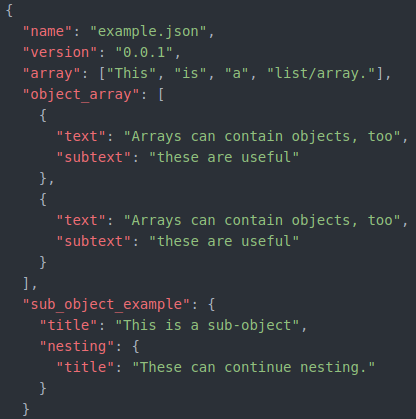
\includegraphics[width=4in]{images/Thesis_JSON.png}
    \caption{JSON excerpt from Beestream's package.json file.}
    \label{fig:json}
 \end{figure}
JSON or JavaScript Object Notation \cite{json} is a data interchange format that is heavily integrated with JavaScript.  The notation is intended to be human-readable, simple, and textual.  It is also used by JavaScript for most object representation.  It is simply constructed of objects that open with a single { (curly brace) followed by a series of comma-separated key-value pairs in the format key : value and closed by a single } (curly brace).  It can also contain lists defined by an opening [ (square bracket) followed by a list of comma separated values or objects and closed with a ] (square bracket).  Part of Beestream’s package.json can be seen in Figure \ref{fig:json} as an example of JSON. This means that JavaScript can be used for anything from data transmission or storage in a web application to human-defined configuration files for web servers and clients.  Due to its simplicity and deep integration into JavaScript, JSON is typically at the core of any JavaScript based application. \par

\subsection{Socket.io & WebSockets}
Socket.io \cite{socket} is a package distributed through NPM that utilizes the WebSocket protocol to offer bi-directional communication channels between a server and a client.  Socket.io provides valuable abstractions for the server and client to setup and communicate through WebSockets.  Socket.io is stable, performs well, and is widely used.  Beestream utilizes Socket.io for most server-client communications due to its simplicity and performance. \par

\subsection{Angular}
Angular \cite{angular} is a client-side application framework built in TypeScript.  TypeScript \cite{typescript} is a strongly typed superscript of JavaScript that compiles into plain JavaScript.  One of Angular’s primary features is its strict enforcement of the MVC architecture with modules, components, and a rendered view.  Angular seeks to provide the developer controlled access to the HTML document and a reliable and secure experience.  Because Angular controls the document, it can provide useful features such as a module-component structure, template-based rendering, and a router to render the appropriate components based on the current URL.  Angular also offers easy support for dynamic content with simple two-way data mapping from the client TypeScript to the rendered document.  Fundamentally, Angular tries to offer a reliable framework for building applications using TypeScript/JavaScript with certain stability and security guarantees.  Other frameworks, such as Vue and React, have seen wide use and can be interchanged with Angular in most applications.  Beestream uses Angular as it’s client-side framework. \par

\subsection{MongoDB}
MongoDB \cite{mongo} is a NOSQL database solution that utilizes BSON (Binary JSON) for data storage.  MongoDB provides a good read-write performance balance and allows for flexibility in the data types and formats that are stored.  Above all, MongoDB integrates well with JavaScript and returns JSON-formatted results that can be immediately accessed and used within a web server or client. \par
